\chapter{Konzeption der Anwendung}
\label{chapter:Konzeption der Anwendung}

\section{Grundidee} 
\label{subsection:Grundidee} 
Bekannte Zusammenhänge zwischen Werten sind meist durch einfache Rechenoperationen umsetzbar. So kann beispielsweise eine Erhöhung der Mehrwertsteuer für ein Produktpreis P mit einer Rechenoperation P = P * M errechnet werden. Für diese Zusammenhänge ist es meist nicht notwendig und sinnvoll, komplexe und vernetzte Softwaresysteme zu entwickeln. 

Wie anfangs erwähnt, wird bei Börsenprognosen der Versuch gestartet, \emph{nicht-lineare Zusammenhänge} innerhalb von Daten zu finden, da lineare und bekannte Zusammenhänge, die zudem noch konstant sind, quasi nicht vorhanden sind. Da neben dieser Anforderung auch die Aktualität und Qualität der Daten eine wichtige Rolle spielt, ist es für die Anwendung sinnvoll und notwendig einen komplexeren und vernetzteren Ansatz für die Realisierung zu verfolgen, auch wenn dies mit einer Steigerung der Kosten einhergehen kann. 

Neben dem Hauptziel, die Zeitreihenextrapolation von Börsendaten, soll außerdem gezeigt werden, wie es konzeptionell und technisch möglich ist, eine derartige Softcomputing-Lösung zu realisieren, welche in einer Systemlandschaft eines Unternehmens mit geringem Aufwand integriert werden kann.

Wichtige Faktoren, die bei der Entscheidung über die Auswahl der eingesetzten Frameworks und Werkzeuge mit eingeflossen sind, ist die Skalierbarkeit, die Wartbarkeit, die Erreichbarkeit sowie die Anschaulichkeit der gewonnen Informationen. 

\subsection{Quandl Data-Provider}
Für Börenprognosen werden quantitative Maßeinheiten benötigt, die im Zusammenhang mit dem betrachteten Kurs stehen. Die wohl Aussagekräftigsten sind Börsenschluss-Index-Werte bzw. Börsenschlusswerte von vergangenen Handelsperioden. Je mehr Daten vorhanden, je realistischer diese Daten sind, desto warscheinlicher ist es, einen Schlusswert in der Zukunft mit Hilfe eines trainierten Neuronalen Netzes vorhersagen zu können. 
Aus diesem Grund spricht die Anwendung, die \emph{Stockmarket-Webapp} den Rest-Service der Quandl-API\footnote[1]{https://www.quandl.com/blog/getting-started-with-the-quandl-api} an.  
Quandl versteht sich als Datenhändler / Datenanbieter mit integrierter Suchfunktion. Das Angebot umfasst die globale Finanzbranche, so z.B. auch sämtliche nationale und internationale Börsenkursdaten der vergangenen Dekaden. 
Die Rest-API bietet die Export-Formate \emph{XML}, \emph{JSON} und \emph{CSV} an.
Somit kann die Anwendung mit echten Börsendaten arbeiten. 


\subsection{Stockmarket-Webapp}
Bei der \emph{Stockmarket-Webapp} handelt es sich um einen Restful-Service, der als Schnittstelle zwischen der Quandl-Rest-API sowie dem Modul der Visualisierung fungiert. Die Stockmarket-Webapp ist das Herzstück der Anwendung und ist u.a. für das testen des Neuronalen Netzes zuständig. Die Aufgabe der Anwendung ist eine schnittstellen - und benutzerdefinierte Datenaufbereitung zu realisieren. Wie das Sequenzdiagramm \emph{Abbilderung-2.1} zeigt, gibt es keine Kommunikation zwischen Fremd-Services, wenn diese nicht über den \emph{ReST-Controller} der Stockmarket-Webapp statt findet. Hierüber können gleich mehrere Vorteile realisiert werden.\\ 
1) Single-Point-Of-Failure: Wenn der Datenlieferant Quandl insolvent geht oder nicht ganz so drastisch, wenn die Anfrage-Mechanismen der Quandl-Rest-API geändert werden, so soll die Anwendung nicht obsolet werden. Ein weiteres Szenario, könnte aus Sicht der Visualisierung einen aus performancebedingten Wechsel der JavaScript-Bibliothek darstellen. Sofern für diese Szenarien keine SPOF-Lösung existiert, würde eine entsprechende Anpassung womöglich ein umfassendes Refactoring aller Anwendungskoponenten erfordern. Im Fall der Stockmarket-Webapp genügt die Anpassung einer Komponente. Will man den Dienst abschalten, so genügt es, die Anwendung zu stoppen.\\   
2) Skalierbarkeit: Den Fall angenommen, weitere Datensätze sollen in weiteren Diagrammen in der Visualisierung dargestellt werden, so ist bereits mit einer einseitigen Anpassung der Visualisierung die Anforderung erfüllt. Der SPOF-Ansatz offeriert Möglichkeiten, die der Skalierbarkeit zuträglich sind. Die Rest-Spezifikation spielt einem hier ebenfalls in die Hände.


\subsection{Visualisierung}
Die Grundidee, die Visualisierung der Anwendungslogik weitgehend von anderen Komponenten zu trennen, hat diverse Vorteile. Die Abhängigkeitsreduktion von diesen Komponenten, das Schaffen einer einheitliche Schnittstelle zwischen den fachlich getrennten Komponenten auch technisch umzusetzen sowie Sicherheitsaspekte spielen dabei eine besondere Rolle.\\
Die Visualisierung ist eine rein clientseitig ausgeführte Anwendung. Diese enthält alle notwendigen Logikroutinen, um Daten anzufragen und entsprechend zu verarbeiten. Die Implementierung dieser Logik wird mit der JavaScript-Bibliothek \emph{jQuery} umgesetzt. Diese manipuliert das Document-Object-Model (DOM) einer HTML-Seite je nach Datenlage. Das DOM kann auch als HTML-Gerüst bezeichnet werden. Für die visuellen Effekte, die eine bessere Veranschaulichung der Graphen ermöglicht, wird die \emph{C3js}-Bibliothek eingesetzt. Um das Layout für Geräte mit unterschiedlicher Displaygröße gleichermaßen nutzbar zu machen, sowie ein dynamisches Layout umzusetzen wird die CSS-Bibliothek \emph{Bootstrap} verwendet. Je weniger Logik in diesem Modul verwendet wird, desto performanter können Datensatze in Diagrammen aktualisiert werden. 

\section{Architektur}
Die Architektur der Anwendung lässt sich mit den erwähnten Technologien, die im folgenden Kapitel besprochen werden entsprechend konstruieren. Das Sequenzdiagramm zeigt den dreigliedrigen Ansatz. 

\begin{figure}[H]
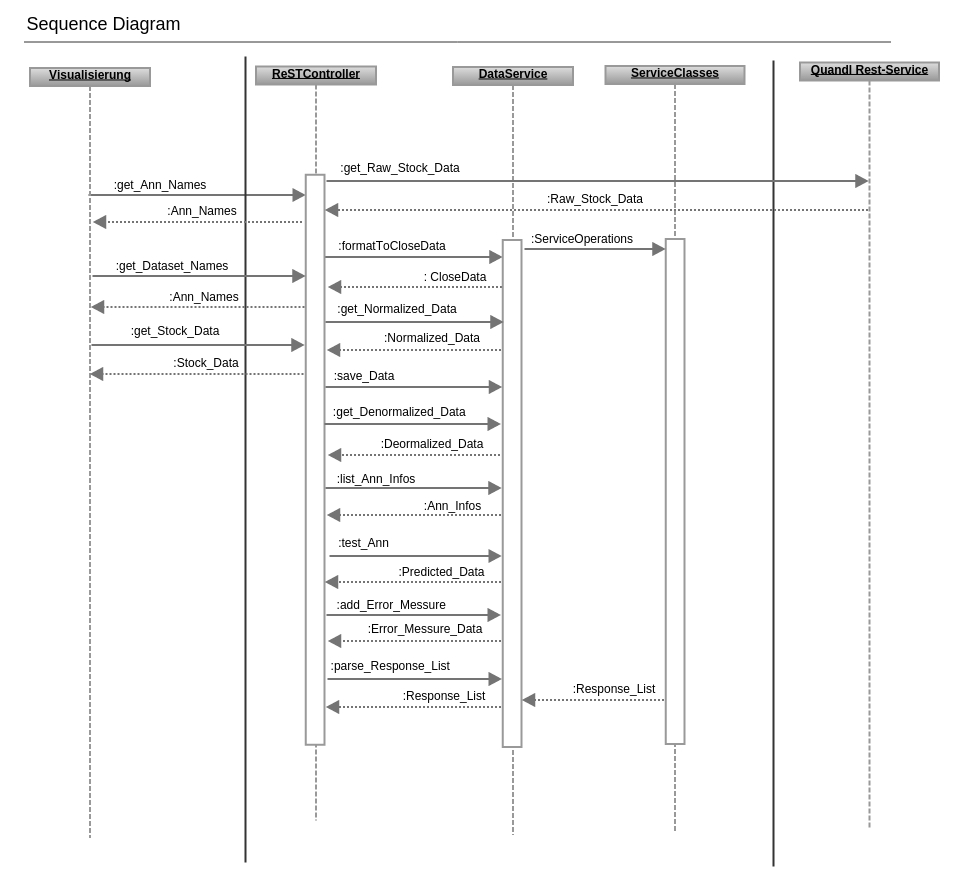
\includegraphics[width=15cm]{Bilder/Konzeption/sequence_dia_rest_env.png}
\captionof{figure}{Sequenzdiagramm - Anwendungslandschaft}
\end{figure}

